\documentclass[11pt]{article}
\usepackage[a4paper,margin=1in]{geometry}
\usepackage[T1]{fontenc}
\usepackage{lmodern,microtype,booktabs,graphicx,amsmath,hyperref,caption,enumitem,xcolor}
\hypersetup{colorlinks=true,linkcolor=blue!50!black,urlcolor=blue!50!black,citecolor=blue!50!black}
\setlength{\parskip}{4pt}
\title{\textbf{An Open, Leak-Controlled Evaluation Pipeline for Fracture Detection:\\Internal Accuracy, External Transfer, and Shortcut Audits}}
\author{Navin Bondade\\University College London\\\texttt{navin.bondade.25@ucl.ac.uk}}
\date{October 2026 \;(preprint draft, not peer reviewed)}
\begin{document}
\maketitle

\begin{abstract}
We build an open pipeline that trains a fracture classifier on public radiographs and audits it for leakage, failure modes and external transfer.
A ConvNeXt-Tiny trained on FracAtlas with a leak-controlled five-fold split reaches an out-of-fold AUC of 0.923 (95\% CI 0.910--0.935).
Scored without retraining on GRAZPEDWRI-DX (20,327 paediatric wrist images, patient-grouped), AUC falls to 0.825, and to 0.697 on initial examinations.
The model flags almost every casted image (sensitivity 0.995, specificity 0.017), a treatment-artefact shortcut invisible in the training data.
We then try to repair the model's weakness on the smallest fractures (sensitivity 0.761 on the smallest quartile) with box-supervised auxiliary heads, a finer localisation head and oversampling.
The outcome is \emph{inconclusive}: the unmodified model changes by $+0.033$ in small-fracture sensitivity between two random seeds, and no box-supervised run beats its no-box control, yet every auxiliary variant has a positive point estimate ($+0.03$ to $+0.07$ against seed 42) and some intervals clear zero against the mean of the two baselines.
Resolving gains of this size needs several seeds per arm, which we did not run. A site-parameterised emergency-department simulation, built on NHS England public inputs with clearly labelled assumptions, illustrates how external performance changes the alert burden.
All results use public data only; this is not a clinical validation.
\end{abstract}

\section{Introduction}
Reported accuracy of fracture-detection models is usually internal, and leakage, shortcut cues and distribution shift are rarely audited together.
We ask three questions with a single reproducible pipeline: (i) how accurate is a commodity classifier under a leak-controlled split; (ii) does it transfer to an unseen dataset, and where does it fail; (iii) can a localisation-based modification reduce misses of small fractures, and can we tell if it does?
The contribution is the evaluation, including its negative findings, not a new architecture.

\section{Data}
\paragraph{FracAtlas (development).} FracAtlas~\cite{Abedeen_2023} contains mixed-body-part radiographs with fracture labels and bounding boxes for fractured images. There are no patient identifiers, so we form groups from perceptual-hash near-duplicates plus consecutive multi-scan runs, and split by group. Subgroups with fewer than 30 positives or negatives (for example hip and shoulder, 10 positives each) are flagged unreliable.
\paragraph{GRAZPEDWRI-DX (external).} GRAZPEDWRI-DX~\cite{Nagy_2022} has 20,327 paediatric wrist images, grouped by patient. It is used for scoring only, with the threshold fixed beforehand. All images come from one scanner, so device shortcuts cannot be tested.
Dataset licences were not verified at the time of writing (see \texttt{docs/DATA\_LICENCES.md}).

\section{Methods}
\paragraph{Model and training.} ConvNeXt-Tiny~\cite{Liu_2022} (timm), single channel, 512\,px, AdamW with one-cycle schedule, mixed precision, batch 16, up to 12 epochs with patience 4. Five-fold out-of-fold evaluation: test fold $k$, validation fold $(k+1)\bmod 5$.
\paragraph{Operating point.} For each fold model the threshold is the score giving 90\% specificity on its validation fold; sensitivity and specificity are reported at that fixed rule, and scores are shifted so zero is the operating point.
\paragraph{Uncertainty.} 95\% group-bootstrap confidence intervals (1000 draws, whole groups resampled); paired bootstrap for differences between runs on identical folds.
\paragraph{Small-fracture subset.} Positives whose box area relative to the image is at or below the 25th percentile (180 images, about 35 per fold). The primary metric is sensitivity there at the fixed threshold.
\paragraph{Box-supervision experiments.} An auxiliary head predicts a map of box locations during training only (removed before saving). The coarse head gives a $16{\times}16$ map (32\,px cells); a fine head uses a feature-pyramid design for a $32{\times}32$ map (16\,px cells). Targets are max-pooled box masks (boxes grown by 16\,px), positive weight 10, with small boxes upweighted. Boxes are used for 100\%, 25\% or 10\% of fractured training images. Controls: the same head supervised on negatives only (no box information), and the plain model with a second seed. A further candidate oversamples smallest-quartile positives $\times3$.
\paragraph{Analysis plan.} The decision rule (small-fracture sensitivity CI lower bound $>0$ versus \emph{both} baseline seeds, AUC not worse than $-0.01$, specificity not worse than $-0.03$, then replication and an external check) is a self-timestamped local file (\texttt{docs/OVERNIGHT\_PROTOCOL.md}), not an external registration. The box 100/25/10\% runs and the no-box auxiliary control had been seen before it was written and are exploratory; only the fine head, its control and oversampling were run afterwards. The rule was tightened once, after the seed-43 baseline appeared. The comparison with the mean of the two baselines was added after seeing the results.

\section{Results}
\subsection{Internal performance}
Out-of-fold AUC is 0.923 (0.910--0.935), sensitivity 0.808 and specificity 0.897. Excluding hardware-flagged images gives 0.915. The hardware flag alone predicts with AUC 0.567 and image-size class with 0.536. Sensitivity on the smallest-fracture quartile is lower than on the largest (72.2\% vs 87.2\%; here ``small'' is defined by the box's longer side, whereas Section~4.4 uses relative box area, which gives 0.761 for the same baseline). Naive and group-controlled splits give 0.931 and 0.923 with overlapping intervals, so leakage inflation is \emph{not demonstrated}.
Grad-CAM~\cite{Selvaraju_2019} peaks fall inside the annotated box for 63.7\% (59.6--67.8) of detected fractures and 29.7\% of missed ones (chance about 3\%). Occluding the fracture lowers the score by 2.42 logits (2.13--2.72) versus $-0.01$ for a control patch, though 86\% of images stay flagged. Saliency supports review, not mechanism.

\subsection{External transfer to GRAZPEDWRI-DX}
\begin{table}[h]\centering\small
\begin{tabular}{lccc}\toprule
Subset & AUC & Sensitivity & Specificity\\\midrule
FracAtlas hand, internal & 0.899 (0.876--0.920) & 0.866 & 0.742\\
GRAZ, all & 0.825 (0.816--0.833) & 0.776 & 0.749\\
GRAZ, no cast, no metal & 0.744 (0.735--0.753) & 0.61 & 0.79\\
GRAZ, initial exams only & 0.697 (0.687--0.707) & 0.540 & 0.790\\
GRAZ, cast present (96\% fractured) & 0.560 & 0.995 & 0.017\\\bottomrule
\end{tabular}
\caption{Internal and external performance at the pre-specified threshold. Prevalence differs (17.6\% vs 67\%), so only AUC, sensitivity and specificity are comparable.}
\end{table}
Casts shift the score regardless of label, an instance of shortcut learning~\cite{Geirhos_2020} of the kind reported for chest radiographs~\cite{Zech_2018}: the mean logit rises by 7.7 for non-fractured casted images and 5.3 for fractured ones, against a fracture effect of about 2.8 among uncasted images. Frontal views are weakest (initial exams: AUC 0.61, sensitivity 31\%, versus lateral 0.79 and 73\%); combining views by maximum or mean did not help (first-visit studies with both views, $n{=}4951$: frontal 0.580, lateral 0.785, max 0.775, mean 0.743). Sensitivity varies by AO class (51\% for 23r-M, the most common, to 79\% for 22r-D). Re-fitting the threshold on GRAZ gives sensitivity 0.673 at 90\% specificity, so the ranking, not only the threshold, transfers poorly.

\begin{figure}[h]\centering
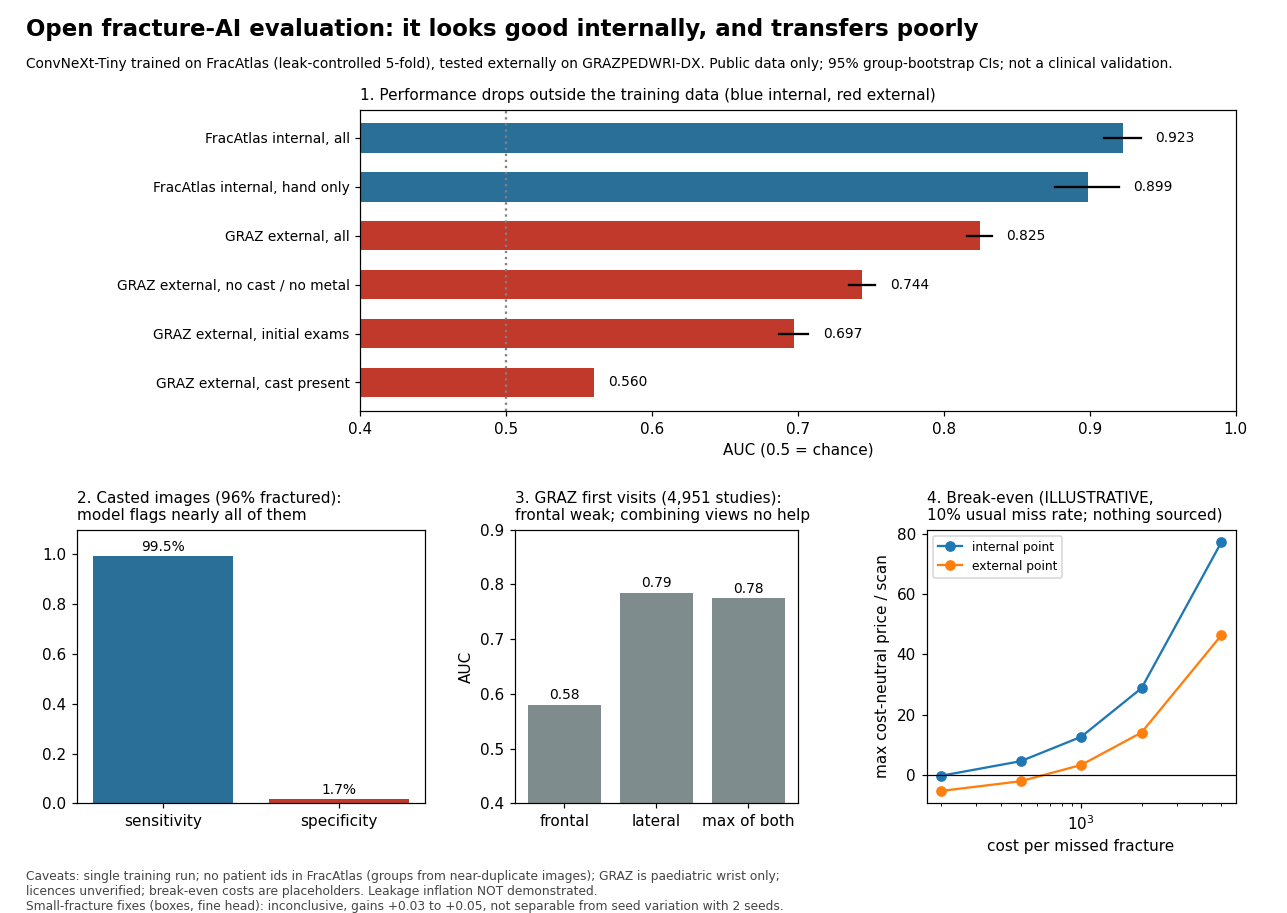
\includegraphics[width=\textwidth]{figures/one_page_summary.png}
\caption{One-page summary of the audit (AUC by subset, cast shortcut, view effect, illustrative break-even).}
\end{figure}

\subsection{Resolution is not the bottleneck}
Downscaling to 384/256/192/128\,px then restoring 512\,px gives AUC 0.919/0.909/0.894/0.850 (native 0.923); sensitivity stays near 0.80 and specificity falls, so blur adds false alarms rather than misses. Upscaling inputs to 640/768\,px gives no gain. Small-fracture sensitivity does not fall with blur. This tests a model trained at 512\,px only.

\subsection{Can missed small fractures be fixed?}
\begin{table}[h]\centering\small
\begin{tabular}{lccl}\toprule
Run & AUC & Small-fracture sens. & Change vs seed-43 baseline\\\midrule
Baseline, seed 42 & 0.923 & 0.761 (0.693--0.822) & --\\
Baseline, seed 43 & 0.932 & 0.794 (0.735--0.854) & (+0.033 vs seed 42)\\
Aux head, no boxes (control) & 0.935 & 0.806 & +0.011 ($-$0.033 to +0.052)\\
Boxes 100\% & 0.936 & 0.833 (0.773--0.885) & +0.039 ($-$0.005 to +0.078)\\
Boxes 25\% & 0.932 & 0.800 & +0.006 ($-$0.043 to +0.051)\\
Boxes 10\% & 0.938 & 0.828 (0.769--0.886) & +0.033 ($-$0.018 to +0.078)\\
Fine head, boxes 100\% & 0.939 & 0.828 (0.770--0.881) & +0.033 ($-$0.013 to +0.080)\\
Fine head, no boxes (control) & 0.936 & 0.794 & +0.000 ($-$0.045 to +0.045)\\
Oversample small $\times3$ & 0.932 & 0.761 (0.688--0.826) & $-$0.033 ($-$0.086 to +0.015)\\\bottomrule
\end{tabular}
\caption{Small-fracture sensitivity at the fixed 90\%-specificity threshold (180 positives). Paired group-bootstrap 95\% intervals.}
\end{table}
Against seed 42 alone, three runs would be called wins (boxes 100\%: $+0.072$, CI $+0.034$ to $+0.119$; boxes 10\%; fine head with boxes). But the unmodified model moved $+0.033$ between seeds, and no box run, compared with its no-box control or with the better baseline (seed 43), has a confidence interval above zero (fine boxes vs fine control: $+0.033$, $-0.010$ to $+0.076$). Oversampling did not help. Against the mean of the two baselines (exploratory, post hoc) three box runs have intervals above zero (boxes 100\%: $+0.056$, $+0.021$ to $+0.090$), and every auxiliary variant has a positive point estimate; the strict rule leans towards the null and the pooled one against it. The seed yardstick is a single pair of runs, so it shows seed variation matters but does not measure it. Any auxiliary head raised overall AUC by about 0.01 with or without boxes, close to the seed difference of $+0.008$. No candidate met the pre-set rule, so replication and the external check were not triggered. The paired 95\% half-width on these 180 images is about 0.045, so differences of about 0.065 or more are detectable in principle, before run-to-run variance; gains of $0.03$ to $0.05$, the size seen here, are not separable from noise with two seeds. A decisive test needs three to five seeds per arm, which were not run.

\subsection{Illustrative break-even}
Treating the model as a safety-net second reader with independence assumed (optimistic), the maximum cost-neutral price per scan is lower at the external initial-exam operating point than the internal one in every cell of a grid of placeholder costs and usual miss rates (for example 3.2 vs 12.6 at a 10\% miss rate and 1,000 per miss) and negative in more cells (11 of 25 external, 5 internal). Costs are not sourced; the point is only that external, not internal, performance decides viability.

\subsection{Illustrative emergency-department simulation}
We built a site-parameterised discrete-event simulation of an ED fracture pathway (\texttt{fracai/twin.py}): limb X-rays arrive with a daytime-peaked pattern, a single reporter works 09 hours a day, and the model acts either as an alert at the time of the X-ray (clinician re-reads flagged images; catch probability 0.8, independence assumed, which is optimistic) or as a triage of the reporting queue. Volume is derived from NHS England's 1.503 million Type~1 attendances in September 2026; everything else is assumed and labelled so: 120 departments, 12\% limb X-ray share (about 49 a day), 20\% fracture prevalence, a 5\% usual miss rate (published studies give roughly 1--4\%), and the model's measured operating points (internal; external first-visit with the external sensitivity on missed fractures scaled by the internal ratio, an assumption). At 5\% miss rate (about 182 missed fractures a year) and a reporter 75\%/95\% busy, an internal-point alert catches about 109 misses before the patient leaves and cuts undetected fracture-hours from 976/1760 to 382/722 a year, at about 12 extra re-reads a day (4 false alarms). The external point catches about 71 and gives 13.5 re-reads a day with 8.2 false alarms. Triage matters most when the reporter is busy. False alerts' harm, costs and patient harm from delay are not modelled. This is an illustration, not a prediction for any hospital. The code includes \texttt{calibrate} and \texttt{validate} steps; on synthetic data generated by the same code, calibration recovered the hidden site and validation passed, which is circular and shows only that the fitting works on a correctly specified model. It would become a digital twin of a real site only after calibration and validation on that site's data.

\section{Related work in brief}
Published small-fracture approaches include a two-stage scaphoid network that re-examines first-stage negatives~\cite{Yoon_2021}, YOLOv8 detectors on GRAZPEDWRI-DX~\cite{Ju_2023} (attention variants of YOLO on the same dataset report gains of about 1--3 mAP50 points, roughly 64\% to 67\%, in papers we did not cite individually), and an object-detection study on paediatric wrist fractures~\cite{Zech_2023}. We have not covered the commercial AI fracture-detection literature, NICE's early value assessment of AI for fracture detection in urgent care, hidden-stratification work, or reporting guidelines (TRIPOD+AI, CLAIM, DECIDE-AI), which a full version should. Differences of that size are comparable to the seed noise we measured; we did not see seed repeats in those reports, but we did not review them exhaustively. This is a brief pointer, not a systematic review.

\section{Limitations}
Single training run per setting, with one extra seed only for the baseline, so run-to-run variance is not estimated. The comparison with the mean of the two baselines is post hoc. The GRAZ overall AUC (0.825) is inflated by the cast shortcut; 0.744 without cast or metal is the fairer headline, and the adult mixed-site to paediatric wrist transfer is partly a task change, not only a domain shift. The ED simulation inputs other than national volume are assumptions. FracAtlas has no patient identifiers, so residual leakage is possible. GRAZ is paediatric wrist only and its \texttt{fracture\_visible} label provenance was not checked. Cast and view analyses are post hoc. Saliency is not evidence of mechanism. Training at higher resolution, a stricter same-bone occlusion control, and training with GRAZ patients included were not tested. Break-even inputs are placeholders. Dataset licences are unverified.

\section{Conclusion}
A commodity classifier that looks strong internally (AUC 0.92) transfers poorly (0.825 overall, 0.744 without cast or metal, 0.697 on first visits) and partly relies on a cast shortcut. Whether box supervision, a finer head or oversampling reduce missed small fractures is \emph{inconclusive}: no variant beats its no-box control, all auxiliary variants move in the positive direction by 0.03 to 0.05, and with two baseline seeds this cannot be told from run-to-run variation. The pipeline's controls stopped three apparent wins against one baseline seed from being reported as findings. The next steps are three to five seeds per arm analysed jointly, a larger small-fracture test set, and site data to calibrate the simulation.

\section*{Reproducibility}
Code, scripts, fixed split files and the analysis plan are in the project repository (\texttt{README.md} gives the run order; 15 unit tests). All runs are resumable and offline.

\bibliographystyle{unsrt}
\bibliography{refs}

\end{document}
